\documentclass[10pt, conference, compsocconf]{IEEEtran}

\usepackage{cite}
\usepackage[pdftex]{graphicx}
\usepackage[cmex10]{amsmath}
\usepackage{algorithmic}
\usepackage{array}

\usepackage{mdwmath}
\usepackage{mdwtab}


\usepackage{eqparbox}
\usepackage[caption=false,font=footnotesize]{subfig}
\usepackage{fixltx2e}
%\usepackage{stfloats}
\usepackage{url}
\usepackage{amssymb}
\usepackage{filecontents}
\usepackage{comment}
\usepackage{url}
\usepackage{balance}
\usepackage{booktabs}
\usepackage[linesnumbered,ruled,vlined]{algorithm2e}

% correct bad hyphenation here
\hyphenation{op-tical net-works semi-conduc-tor}


\begin{document}
%
% paper title
% can use linebreaks \\ within to get better formatting as desired
\title{On Speeding-up Parallel Jacobi Iterations for SVDs}


% author names and affiliations
% use a multiple column layout for up to two different
% affiliations

\author{\IEEEauthorblockN{Soumitra Pal \qquad Sudipta Pathak \qquad Sanguthevar Rajasekaran}
\IEEEauthorblockA{Computer Science and Engineering, University of Connecticut\\
371 Fairfield Road, Storrs, CT 06269, USA\\
\texttt{\small \em \{mitra@,sudipta.pathak@,rajasek@engr.\}uconn.edu}}}

% conference papers do not typically use \thanks and this command
% is locked out in conference mode. If really needed, such as for
% the acknowledgment of grants, issue a \IEEEoverridecommandlockouts
% after \documentclass

% for over three affiliations, or if they all won't fit within the width
% of the page, use this alternative format:
% 
%\author{\IEEEauthorblockN{Michael Shell\IEEEauthorrefmark{1},
%Homer Simpson\IEEEauthorrefmark{2},
%James Kirk\IEEEauthorrefmark{3}, 
%Montgomery Scott\IEEEauthorrefmark{3} and
%Eldon Tyrell\IEEEauthorrefmark{4}}
%\IEEEauthorblockA{\IEEEauthorrefmark{1}School of Electrical and Computer Engineering\\
%Georgia Institute of Technology,
%Atlanta, Georgia 30332--0250\\ Email: see http://www.michaelshell.org/contact.html}
%\IEEEauthorblockA{\IEEEauthorrefmark{2}Twentieth Century Fox, Springfield, USA\\
%Email: homer@thesimpsons.com}
%\IEEEauthorblockA{\IEEEauthorrefmark{3}Starfleet Academy, San Francisco, California 96678-2391\\
%Telephone: (800) 555--1212, Fax: (888) 555--1212}
%\IEEEauthorblockA{\IEEEauthorrefmark{4}Tyrell Inc., 123 Replicant Street, Los Angeles, California 90210--4321}}



% make the title area
\maketitle


\begin{abstract}
We live in an era of big data and the analysis of these data is becoming a bottleneck in many domains including biology and the internet. To make these analyses feasible in practice, we need efficient data reduction algorithms. The Singular Value Decomposition (SVD) is a data reduction technique that has been used in many different applications. For example, SVDs have been extensively used in text analysis. Several sequential algorithms have been developed for the computation of SVDs. The best known sequential algorithms take cubic time which may not be acceptable in practice. As a result, many parallel algorithms have been proposed in the literature. There are two kinds of algorithms for SVD, namely, QR decomposition and Jacobi iterations. Researchers have found out that even though QR is sequentially faster than Jacobi iterations, QR is difficult to parallelize. As a result, most of the parallel algorithms in the literature are based on Jacobi iterations. JRS is an algorithm that has been shown to be very effective in parallel. JRS is a relaxation of the classical Jacobi algorithm. In this paper we propose a novel variant of the classical Jacobi algorithm that is more efficient than the JRS algorithm. Our experimental results confirm this assertion. We also provide a convergence proof for our new algorithm. We show how to efficiently implement our algorithm on such parallel models as the PRAM and the mesh. 
\end{abstract}

\begin{IEEEkeywords}
SVD; Jacobi iterations; JRS; parallel algorithms
\end{IEEEkeywords}


% For peer review papers, you can put extra information on the cover
% page as needed:
% \ifCLASSOPTIONpeerreview
% \begin{center} \bfseries EDICS Category: 3-BBND \end{center}
% \fi
%
% For peerreview papers, this IEEEtran command inserts a page break and
% creates the second title. It will be ignored for other modes.
\IEEEpeerreviewmaketitle



\section{Introduction}
\label{sec:intro}

Singular Value Decomposition (SVD) is a fundamental computational problem in linear algebra and it has application in various computational science and engineering areas. For example, it is widely used in areas such as statistics where it is directly related to principal component analysis, in signal processing and pattern recognition as an essential filtering tool, and in control systems. Recently, it is used as one of the fundamental steps in many machine learning applications such as least square regressions, information retrieval and so on. With the advent of BigData, it has become essential to process data matrices with thousands of rows and columns in real time. The SVD is one of the data reduction techniques. Hence, there is a strong need for efficient sequential and parallel algorithms for the SVD.

SVD takes as input a matrix $A \in \mathbb{F}^{m \times n}$ where $\mathbb{F}$ could be the field of real ($\mathbb{R}$) or complex ($\mathbb{C}$) numbers and outputs three matrices $U, S, V$ such that $A = USV^T$, where $U \in \mathbb{F}^{m \times m}$, $V \in \mathbb{F}^{n \times n}$ are orthogonal matrices (i.e. $U^TU = I_m$, $V^TV = I_n$) and $S \in \mathbb{R}^{m \times n}$ is a diagonal matrix. If $S = diag(\sigma_1, \sigma_2,......\sigma_{\min\{m,n\}})$, then the diagonal elements $\sigma_i$s are called the singular values of $A$. The columns of $U$ and $V$ are referred to as the left and right singular vectors respectively. Without loss of generality, we assume that $m \ge n$. We also assume that the input matrices are real, the algorithms in this paper can be easily extended to complex matrices. 

There are various methods of computing the SVD~\cite{golub2012matrix}. The most commonly used algorithms for dense matrices, which we consider in this paper, can be classified as \emph{QR-based} and \emph{Jacobi-based}. The QR-based algorithms work in two stages. In the first stage the input matrix is converted to a band matrix (bidiagonal, tridiagonal and so on) using factorizations such as Cholesky, LU and QR. In the final stage the band matrix is converted to a diagonal form to obtain the singular values. The singular vectors are also computed accordingly. In the sequential setting, the QR based methods are more frequently used as they are faster than the sequential Jacobi based methods. However, Jacobi-based methods are known to be more accurate~\cite{demmel1992jacobi} and also have a higher degree of potential parallelism. Though there are parallel implementations of QR based algorithms in out-of-core setting~\cite{grimes1987solution, grimes1988solution} as well as in homogeneous multi-core setting~\cite{haidar2013improved}, our focus is on designing faster parallel implementations of the Jacobi based algorithms.

There are two different variations of the Jacobi based algorithms, \emph{one-sided} and \emph{two-sided}. The two sided Jacobi algorithms are applicable only when $A$ is symmetric and $m=n$. The basic idea of a two sided Jacobi algorithm is as follows. Using a series of plane rotation matrices $U_1, U_2, \ldots, U_t$, the symmetric matrix $A$ is converted a diagonal matrix $S = U_t \ldots U_2 U_1 A U^T_1 U^T_2 \ldots U^T_t$. The left and right singular vectors are given by $U=V=U_1U_2,\ldots,U_t$. The basic idea of the one-sided Jacobi algorithms proposed by Hestenes~\cite{hestenes1958inversion} is as follows. Using a series of plane rotation matrices $V_1, V_2, \ldots, V_t$ the input matrix $A$ is first converted to a matrix $B=AV_1V_2\ldots V_t$ such that the columns of $B$ are orthogonal. The decomposition $B = US$ gives us the required left singular vectors and the singular values respectively, where $U$ is obtained by normalizing the columns of $B$ (keeping null columns unchanged) and the norm of $i$th column of $B$ gives $S_{ii}$ of the diagonal matrix $S$. The right singular vectors are the columns of $V=V_1V_2,\ldots,V_t$. As the rotation matrices $V_i$s are orthogonal, $V$ is also orthogonal and hence $AV = B = US$ implies $A = USV^T$.

Each of the plane rotation matrices $V_i$ corresponds to a pair of columns $(j,k)$ where the rotation is on the plane going through the $j$th and the $k$th axes. We assume $j<k$ and call such a pair $(j,k)$ a \emph{pivot}.  In the traditional Jacobi algorithms the rotations are divided among \emph{sweeps}, in each sweep all possible ${n \choose 2}$ pivots are used. For the one-sided Jacobi, the rotation using pivot $(j,k)$ annihilates the off diagonal entries $a_{jk}, a_{kj}$ to $0$. However, either of $a_{jk}, a_{kj}$ may again become non-orthogonal due to some later pivot involving $j,k$ in the same sweep. Hence multiple sweeps are required. As a test for convergence, we could check if the Frobenius norm of the off-diagonal entries of $A$ fell below a certain tolerance. For the two-sided Jacobi, pivoting $(j,k)$ ensures that the columns $a_j,a_k$ become mutually orthogonal after the rotation. Here too, multiple sweeps may be required as the columns may again become non-orthogonal due to some later pivot. For convergence, we could count how many times in any sweep the dot-product $a_j^{T}a_k$ fell below a certain tolerance and the algorithm is terminated when the count reached $n(n-1)/2$. It is believed that the number $S$ of sweeps needed for the convergence of the sequential one-sided and two-sided Jacobi algorithm is $O(\log n)$~\cite{golub2012matrix}.  

It turns out that order in which the pivots are applied in a sweep has a significant effect on the number of sweeps required for convergence. Mainly two different orders are used. In the classic Jacobi algorithm~\cite{golub2012matrix}, each rotation chooses the pivot $(j,k)$ with maximum absolute value of $a_{jk}$ in the two-sided Jacobi and the maximum value of the dot-product $a_j^{T}a_k$ in the one-sided Jacobi. However, searching for this element is computationally expensive. Cyclic Jacobi algorithms trade off this computation with slower convergence and uses the pivots in the order $(1,2), (1,3), \ldots, (1,n), (2,3), (2,4), \ldots, (2,n), \ldots (n-1,n)$.  It can be shown that after each sweep in one-sided Jacobi the Frobenius norm of off-diagonal entries reduces monotonically and hence the algorithm converges. For the two-sided Jacobi the sum of dot-products of all pairs of columns reduces in each sweep.

Many pivots in a sweep are independent of each other and hence the corresponding rotations can be applied in parallel. In fact the sweeps can be divided into $(n-1)$ \emph{subsweeps} each containing $n/2$ independent pivots and all rotations in a subsweep can be applied in parallel. There are many ways of dividing the pivots in a subsweep. A simple round-robin based ordering is given in~\cite{golub2012matrix}. However, it turns out that more clever pivot ordering improves performance by reducing the total number of sweeps required for convergence~\cite{becka2002dynamic}.

\subsection{Contributions}

In this paper we introduce a novel algorithm for parallel computation of SVDs. This algorithm uses the idea of picking the pivots in the order of maximum absolute value of $a_{jk}$ in two-sided Jacobi and of $a_j^T a_k$ in one-sided Jacobi. However, to reduce the high computational cost of searching for the maximum before each rotation, the algorithm uses two relaxations. 1) Instead of searching for the maximum before each iteration, the pivots are sorted in descending values of $a_{jk}$ or $a_j^T a_k$ at the beginning of a sweep and the pivots are applied in this order. 2) To reduce the quadratic sorting time, only the top $1/k$th of the pivots are selected and they are applied in the sorted order. We call this JPS (Jacobi Pivot Sorting) scheme hereafter. Our contributions are as follows. Firstly we show using a simulation based technique~\cite{rajasekaran2008relaxation} that the JPS scheme significantly reduces the number of sweeps. Secondly we give a `real' implementation of our ideas in a one-sided Jacobi algorithm based on the code from Gnu Scientific Library~\cite{galassi1996gnu}. We also give a parallel implementation in the shared memory multi-core setting. Finally we discuss the implementation of JPS scheme on various models of computing such as the mesh, the hypercube, and the PRAM.
 

The remainder of the paper is organized as follows: In Section~\ref{sec:prevwork}, we survey the previous work on Jacobi-SVD algorithm.  Section~\ref{sec:jps} describes our new JPS algorithm. In Section~\ref{sec:results}, we show experimental results. Section~\ref{sec:other} discusses implementations of our new algorithms in different models of parallel computing. Finally, we provide some concluding remarks in Section~\ref{sec:conclude}.

\section{A Survey of Basic Ideas}
\label{sec:prevwork}

Most existing parallel algorithms for SVD are based on the Jacobi iterations. At the heart of these iterations is the Jacobi rotation (also known as Givens rotation~\cite{golub2012matrix}). A rotation of angle $\theta$ in the plane going through the axes $j,k$ can be represented as the following matrix:
%\begin{figure}
\begin{align}
  J(j,k,\theta) &= \left( \begin{array}{ccccccc} 
  1 & \cdots & 0 & \cdots & 0 & \cdots & 0 \\
  \vdots & \ddots & \vdots & & \vdots & & \vdots \\
  0 & \cdots & c & \cdots & s & \cdots & 0 \\
  \vdots & & \vdots & \ddots  & \vdots & & \vdots \\
  0 & \cdots & -s & \cdots & c & \cdots & 0 \\
  \vdots & & \vdots & & \vdots  & \ddots  & \vdots \\
  0 & \cdots & 0 & \cdots & 0 & \cdots & 1
\end{array} \right)
\begin{array}{l}
  \\
  j \\
  \\
  k
  \\
  \\
\end{array} \\
& \begin{array}{ccccccc}
 \qquad &\qquad & j & \qquad & k & &
\end{array} \nonumber
\end{align}
%\end{figure}
where $c=\cos \theta$ and $s=\sin \theta$. It is easy to verify that $J^T J = I$, so Jacobi rotation is an orthogonal
transformation.

\subsection{Sequential algorithms}

The two-sided Jacobi algorithms attempts to diagonalize the input matrix $A$ by applying a series of Jacobi rotations of the form $B = J^T A J$. It can be easily verified that if $A$ is symmetric then $B$ is also symmetric. Suppose we need to annihilate the element $a_{jk}$ (by symmetry $a_{kj}$ too), then the effects of the transformation on elements $b_{jj}, b_{jk}, b_{kj}, b_{kk}$ can be written in the matrix form as follows:
\begin{align}
\setlength{\arraycolsep}{2.5pt}
  \left(\begin{array}{cc}
    b_{jj} & b_{jk} \\
    b_{kj} & b_{kk}
  \end{array} \right)
  =
  \left(\begin{array}{cc}
    c & s \\
    -s & c
  \end{array} \right)^T
  \left(\begin{array}{cc}
    a_{jj} & a_{jk} \\
    a_{kj} & a_{kk}
  \end{array} \right)
  \left(\begin{array}{cc}
    c & s \\
    -s & c
  \end{array} \right).
\end{align}
Solving for $b_{jk} = b_{kj} = 0$ and taking the smaller root~\cite{golub2012matrix}, gives 
\begin{align}
  c &= \frac{1}{\sqrt{1+t^2}}, & s&=tc, \qquad \text{where} \nonumber \\
  t &= \frac{sign(\gamma)}{|\gamma|+\sqrt{\gamma^2+1}}, & \text{and} \quad \gamma &= \frac{a_{kk} - a_{jj}}{2a_{jk}}.
\end{align}

The one-sided Jacobi algorithm, also called Hestenes–Jacobi algorithm~\cite{hestenes1958inversion}, converts the input matrix $A$ to a orthogonal matrix $B$ using a series of Jacobi rotations. For a pivot $(j,k)$ the rotation affects only the columns $j,k$ and can be written in the following matrix notation:
\begin{align}
\setlength{\arraycolsep}{2.5pt}
  \left(\begin{array}{cc}
    b_{j} & b_{k} 
  \end{array} \right)
  =
  \left(\begin{array}{cc}
    a_{j} & a_{k} 
  \end{array} \right)
  \left(\begin{array}{cc}
    c & s \\
    -s & c
  \end{array} \right).
\end{align}
The two columns would be orthogonalized if $b_j^T b_k = 0$. Thus solving for $b_{j}^T b_{k} = 0$ gives the solution 
\begin{align}
  c &= \frac{1}{\sqrt{1+t^2}}, & s&=tc, \qquad \text{where} \nonumber \\
  t &= \frac{sign(\gamma)}{|\gamma|+\sqrt{\gamma^2+1}}, & \text{and} \quad \gamma &= \frac{a_k^T a_k - a_j^T a_j}{2a_j^Ta_k}.
\end{align}
As we could see, there is a close similarity between the one-sided and two-sided versions of the Jacobi algorithm, the one-sided algorithm could be thought of as applying two-sided algorithm on the symmetric matrix $A^TA$. In the rest of the paper we will refer to the one-sided algorithm only as it handles more general matrices and is mostly used in the literature.

\subsection{Parallel algorithms}



\cite{bevcka2013parallel, kudo2016parallel, becka2015parallel} introduced and implemented the idea of parallel one-sided block jacobi algorithm with dynamic ordering and variable blocking. Their approach, known as OSBJ method, accomplishes the parallel SVD in three stages namely, pre-processing, iteration and post processing. There are two types of pre-processing depending on the dimension of the matrix, namely QR-pre-processing and LQ pre-processing. During QR-pre-processing OSBJ decomposes input matrix $A = Q_1R$ where $A \in \mathbb{R}^{m \times n}$, orthonormal matrix $Q_1 \in \mathbb{R}^{m \times m}$ and upper triangular matrix $R \in \mathbb{R}^{n \times n}$. On the contrary, LQ-pre-processing decomposes input matrix $A = LQ_2$ where $L \in \mathbb{R}^{n \times n}$ is a lower triangular matrix and $Q_2 \in \mathbb{R^{n \times n}}$ is an orthogonal matrix. The $L$ or $R$ matrix in pre-processing stage is considered as input $A^0$ for the iteration stage.
$A^0$ is partitioned into column blocks. Let, $A^{(r)}_i$ and $A^{(r)}_j$ are one such column block pair where $1 \leq i < j \leq l$ assuming we have $l$ such column blocks. Weight $\hat{w}^{r}_{ij} = \frac{||{A^{(r)}_i}^TA^{(r)}_j\textbf{e}||_2}{||\textbf{e}||_2}$, where $\textbf{e} = (1, 1, ....1)^T \in \mathbb{R}^{\frac{n}{l}}$.  $\hat{w}^{r}_{ij}$ serves as an approximate measure of inclination between $Im(A^{r}_i)$ and $Im(A^{r}_j)$. The column block pairs are ordered based on their mutual inclination and the most mutually inclined pair is chosen to be orthogonalized and those columns are excluded from the set for next iteration. The process is repeated until all the column blocks are used up. For each column block pair a $2 \times 2$ Gram matrix $G_s \in \mathbb{R}^{\frac{2n}{l} \times \frac{2n}{l}}$ is constructed as is given by $G_s = [A^{(r)}_{i_{r,s}},A^{(r)}_{j_{r,s}}]^T[A^{(r)}_{i_{r,s}},A^{(r)}_{j_{r,s}}]$ where $1 \leq s \leq \frac{l}{2}$. This gram matrix is them diagonalized as $G_s = V_sD_sV_s^T$ where $V_s$ is an orthogonal matrix and $D_s$ is a diagonal matrix. The column blocks for next iteration $A^{(r+1)}$ is computed by $[A^{(r+1)}_{i_{r,s}},A^{(r+1)}_{j_{r,s}}] = [A^{(r)}_{i_{r,s}},A^{(r)}_{j_{r,s}}]V_s$. Iteration process continues until all the columns are mutually orthogonal. 
\par The Jacobi Relaxation Scheme (JRS) algorithm by Rajasekaran and Song introduced the idea of improving parallelism in SVD computation by 
multiplying the off-diagonal element in each iteration by a very small number $\epsilon$ such that $0 < \epsilon < 1$ instead of setting the off-diagonal element to zero. \cite{rajasekaran2008relaxation} compares number of iterations taken by JRS algorithm to converge with that of Strumpen's Independent Jacobi algorithm \cite{strumpen2003stream} and shows that JRS takes much less number of iterations to converge than Independent Jacobi. 

This paper has done same parallel implementation:~\cite{soliman2008memory}.

This paper seems to do some kind of sorting for~\cite{zhou1995parallel}.
Since any rotation in the two-sided Jacobi algorithm changes
only the corresponding (two) rows and (two) columns, and
771
one-sided Jacobi algorithm changes only the corresponding
(two) rows, there exists inherent parallelism in the Jacobi
iteration algorithms. For example, the n(n − 1)/2 rotations in
any sweep can be grouped into n −1 rotation sets each of which
contains n/2 independent rotations. For instance, if n = 4, there
are three rotation sets: {(1,2),(3,4)}, {(1,3),(2,4)}, {(1,4),(2,3)}.
Since each rotation can be performed in O(n) time on a single
machine, we can perform all the rotations in O(n 2 S) time on a
ring of n processors [6]. The idea here is to perform each set of
rotations in parallel.
We can think of the Jacobi algorithm as consisting of two
phases. In the first phase we compute all the rotation matrices
(there are O(n 2 ) of them). In the second phase we multiply
them out to get U and V . Consider any rotation operation. The
values of s and c can be computed in O(1) time sequentially.
The algorithm of Strumpen et al. [11] performs all the n(n −
1)/2 rotations of a sweep in parallel even though not all of
these rotations are independent. Thus in their algorithm, all
the rotation matrices can be constructed in O(1) time using
n 2 CREW PRAM processors. This will complete the first
phase of the Jacobi algorithm. The second phase has to be
completed. This involves the multiplication of O(n 2 ) rotation
matrices. Since two n×n matrices can be multiplied in O(log n)
time using n 3 CREW PRAM processors (see e.g. [4,8]), a
straightforward implementation of [11]’s algorithm runs in time
O(S log 2 n) using n 5 CREW PRAM processors. In [11] an
implementation on an n × n mesh has been given that runs
in O(nS) time. However, as has been pointed out before, the
value of S is much larger than the corresponding value for the
sequential Jacobi iteration algorithm.
Any parallel algorithm for SVD partitions the n(n − 1)/2
rotations of a sweep into rotation sets where each rotation
set consists of a number of rotations. All the rotations of a
rotation set are performed in parallel. Most of the parallel
SVD algorithms in the literature employ (n − 1) rotation sets
each rotation set consisting of n/2 independent rotations. The
algorithm of Strumpen et al. is an exception, where multiple
processors compute the rotation matrices independently, all
the processors employing the same original matrix. In the
sequential case, if A is the input matrix, computations will
proceed as follows: B 1 = J 1 T A J 1 ; B 2 = J 2 T B 1 J 2 ; B 3 =
J 3 T B 2 J 3 ; and so on. On the other hand, in parallel, computations
will proceed as follows: B 1 = J 1 T A J 1 ; B 2 = J 2 T A J 2 ; B 3 =
J 3 T A J 3 ; etc. The number of B i s computed in parallel will
be decided by the number of available processors. Once
this parallel computation is complete, all of the computed
transformations will be applied to A to obtain a new matrix
B. After this, again a parallel computation of rotation matrices
will be done all with respect to B; B will be updated with the
computed transformations; and so on.
In this paper we propose a fundamentally different algorithm
for SVD. It is a specific “relaxation” of the Jacobi iteration
algorithm called JRS iteration algorithm. Just like the Jacobi
algorithm, there are two variants of the JRS iteration algorithm
as well, namely, one-sided and two-sided. We provide details
on these two variants in the next subsections.


3.1. Two-sided JRS iteration algorithm
The main idea behind the original two-sided Jacobi SVD is
to systematically reduce the norm of the off-diagonal elements
of a symmetric matrix A:
n
n
a i 2 j .
off(A) =
i=1 i=1, j=i
The convergence of the Jacobi algorithm is ensured by the fact
that after each rotation, the norm of the off-diagonal elements
decreases by twice the square of the element zeroed out in this
rotation [6].
The JRS iteration algorithm also has sweeps and in each
sweep we perform rotations (one corresponding to each off-
diagonal element). The only difference is that in a given rotation
we do not zero-out the targeted off-diagonal element but rather
we decrease the value of this element by a fraction.
Let the element targeted in a given rotation be the (i, j)th
element. Then we let
b i j = a i j (c 2 − s 2 ) + (a ii − a j j )cs = λa i j ,
where λ is in the interval [0, 1). When λ = 0, we obtain the
original Jacobi iteration algorithm. We can solve for s and c as
follows: If a i j = 0, then set c = 1 and s = 0; Otherwise
a ii − a j j
c
s
λ
=
−
−
.
2a i j
2s
2c 2cs
Let τ =
a j j −a ii
2a i j
, t = c s , then
(1 + λ)t 2 + 2τ t + λ − 1 = 0.
According to [6], the smaller root should be chosen, so
sign(τ )(1 − λ)
t =
|τ | +
τ 2 + (1 − λ 2 )
.
Like in the regular Jacobi rotation, c and s can be computed as:
c = √
1
1 + t 2
,
s = tc.
We call the above algorithm JRS iteration algorithm.
Depending on whether it is implemented in sequence or in
parallel, there are two variants: JRS sequential algorithm
and JRS parallel algorithm. In sequential version, we
compute another rotation after applying the rotation previously
computed; In a parallel algorithm, we can compute all n(n −
1)/2 rotations of a sweep independently and then apply these
rotations altogether. They are described in the following pseudo
codes:
JRS sequential algorithm (A, λ, )
//A: Input matrix, λ: relaxation parameter, : convergence
scale.
δ = × A
B := A;
2 ;
F
Repeat
{
for i = 1 to n − 1 do
{
for j = i + 1 to n do
{
Compute Jacobi rotation parameters (c,s) with respect
to B i j for B using the formulas in Section 3.1;
Let J i j be the corresponding rotation matrix;
B := J i T j B J i j ;
}
}
Compute the squared off-diagonal norm of B; Let it be f ;
} until ( f < δ);
JRS parallel algorithm (A, λ, )
//A: Input symmetrical matrix, λ: relaxation parameter, :
convergence scale.
δ = × A 2 F ;
B := A;
Repeat
{
for i = 1 to n − 1 do in parallel
{
for j = i + 1 to n do in parallel
{
Compute Jacobi rotation parameters (c,s) with respect
to B i j for B using the formulas in Section 3.1;
Let J i j be the corresponding rotation matrix;
}
}
T
T
T B J ··· J
B := J (n−1)n
J (n−2)n
· · · J 12
12
(n−2)n J (n−1)n ;
Compute the squared off-diagonal norm of B; Let it be f ;
} until ( f < );
We can prove the convergence of JRS sequential algorithm
in a similar manner to that of the Jacobi algorithm. In particular,
we can show that after each rotation the norm of the off-
diagonal elements decreases by a constant multiple of the
square of the targeted element. However, as in the regular
Jacobi algorithm, it is difficult to estimate the number of
sweeps needed for convergence. Also, it is hard to prove the
convergence of JRS parallel algorithm in theory.
Convergence: We can show that the sequential JRS algorithm
converges in the limit in exactly the same way we prove the
convergence of the sequential Jacobi algorithm. Let A be a
given n × n symmetrical matrix and consider any rotation
J (i, j, θ ). As explained in Section 2.1, A gets modified as
B = J T A J due to the rotation J (i, j, θ ). Since the Frobenius
norm is preserved under orthogonal transformations, it is the
case that a ii 2 +a 2 j j +2a i 2 j = b ii 2 +b 2 j j +2b i 2 j = b ii 2 +b 2 j j +2λ 2 a i 2 j .
n
n
Therefore, off(B) 2 = B 2 − i=1
b ii 2 = A 2 − i=1
a ii 2 +
(a ii 2 + a 2 j j − b ii 2 − b 2 j j ) = off(A) 2 − 2(1 − λ 2 )a i 2 j .


One-sided JRS algorithm is similar to the two-sided
Jacobi algorithm. In each rotation, we let the norm of the
corresponding two rows be reduced to a fraction of it. That is,
v i T v j = λu i T u j .
The solution is similar to the two-sided Jacobi
1
c = √
,
s = tc.
1 + t 2
where
sign(τ )(1 − λ)
,
t =
|τ | + τ 2 + (1 − λ 2 )
and
τ =
u T j u j − u i T u i
2u i T u j
.
3.3. Group JRS iteration algorithm
In this section we present a variant of the JRS algorithm.
The JRS iteration algorithm is such that all the rotations in a
sweep are performed independently and in parallel. The number
of sweeps for convergence is small. Thus JRS algorithm is
amenable to maximum parallelism. For example, we can obtain
a cost optimal algorithm using upto n 2 processors on a variety
of models of computing.
As described before, there are n(n − 1)/2 rotations in a
sweep. These rotations can be grouped into n − 1 rotation sets
each of which containing n/2 nonconflicting rotations. Given
that all the rotations of a sweep can be performed in parallel in
the case of the JRS algorithm, a variant of the JRS algorithm
can be devised as follows: We partition the n − 1 rotation sets
into g groups (for some appropriate value of g), each group
n
n−1
having n−1
g sets. We compute all the ( 2 × g ) rotations in one
group in parallel using the JRS algorithm. It is true that there are
conflicts among the rotations of any group, but the relaxation
scheme helps in reducing the convergence time. Thus all the
rotations of a sweep can be completed in g parallel steps. We
call this variant as the Group JRS Algorithm, which is described
in the following pseudo code:
Group JRS Parallel Algorithm (A, λ, )
//A: Input matrix, λ: relaxation parameter, : convergence
scale.
δ = × A 2 F ;
B := A;
Repeat
{
for each group G do
{
for each element in G do
{
Compute Jacobi rotation parameters (c, s) with respect
to this element for B;
}
Apply all the rotation matrices computed for G on B and
update B;
}
Compute the squared off-diagonal norm of B; Let it be f ;
} until ( f < );

\section{JPS Algorithm}
\label{sec:jps}

\begin{algorithm}
\KwIn{Matrix $A$, selection parameter $\tau$, \newline convergence scale $\epsilon$}
\KwOut{SVD matrices $U, S, V$}
$\delta \gets \epsilon \times ||A||^2_F$; \quad $B \gets A$; \quad $V \gets I_n$\;
\Repeat{maximum sweeps is reached}{
  $P \gets $ empty array of pivot tuples $(j,k,b^T_j b_k)$\;
  \For{$j \gets 1$ \textbf{to} $n-1$} {
    \For{$k \gets j+1$ \textbf{to} $n$} {
      insert $(j, k, b^T_jb_k)$ in P\; 
    }
  }
  sort $P$ in descending values of dot-products\;
  \If{largest dot-product in $P$ is $< \delta$}{
    compute singular values $S$ and singular vectors $U$ from $B$ as explained in Section~\ref{sec:intro}\;
    \Return $U,S,V$\;
  }
  \For{$i \gets 1$ \textbf{to} $n(n-1)/(2\tau)$} {
      $(j,k,d) \gets P[i]$\;
      compute Jacobi rotation parameters $(c,s)$ with respect to $B_{jk}$ for B using formulas in Section~\ref{sec:prevwork}\;
      let $J_{jk}$ be corresponding rotation matrix\;
      $B \gets B J_{jk}$; \quad $V \gets V J_{jk}$\;  
  }
}
\caption{One-sided Sequential JPS}
\label{algo:seqjps}
\end{algorithm}


\begin{algorithm}
\KwIn{Matrix $A$, selection parameter $\tau$, \newline convergence scale $\epsilon$}
\KwOut{SVD matrices $U, S, V$}
$\delta \gets \epsilon \times ||A||^2_F$; \quad $B \gets A$; \quad $V \gets I_n$\;
\Repeat{maximum sweeps is reached}{
  $P \gets $ empty array of pivot tuples $(j,k,b^T_j b_k)$\;
  \For{$j \gets 1$ \textbf{to} $n-1$} {
    \For{$k \gets j+1$ \textbf{to} $n$} {
      insert $(j, k, b^T_jb_k)$ in P\; 
    }
  }
  sort $P$ in descending values of dot-products\;
  \If{largest dot-product in $P$ is $< \delta$}{
    compute singular values $S$ and singular vectors $U$ from $B$ as explained in Section~\ref{sec:intro}\;
    \Return $U,S,V$\;
  }
  $Q \gets$ empty queue of Jacobi rotation matrices\;
  \For{$i \gets 1$ \textbf{to} $n(n-1)/(2\tau)$} {
      $(j,k,d) \gets P[i]$\;
      compute Jacobi rotation parameters $(c,s)$ with respect to $B_{jk}$ for B using formulas in Section~\ref{sec:prevwork}\;
      let $J_{jk}$ be corresponding rotation matrix\;
      push $J_{jk}$ in $Q$\;
  }
  \While{not empty $Q$}{
    pop $J$ from $Q$\;
    $B \gets BJ$; \quad $V \gets VJ$\;  
  }
}
\caption{One-sided Simulated Parallel JPS}
\label{algo:simjps}
\end{algorithm}


\begin{algorithm}
\KwIn{Matrix $A$, selection parameter $\tau$, \newline convergence scale $\epsilon$}
\KwOut{SVD matrices $U, S, V$}
$\delta \gets \epsilon \times ||A||^2_F$; \quad $B \gets A$; \quad $V \gets I_n$\;
\Repeat{maximum sweeps is reached}{
  $P \gets $ empty array of pivot tuples $(j,k,b^T_j b_k)$\;
  \For{$j \gets 1$ \textbf{to} $n-1$} {
    \For{$k \gets j+1$ \textbf{to} $n$} {
      insert $(j, k, b^T_jb_k)$ in P\; 
    }
  }
  sort $P$ in descending values of dot-products\;
  \If{largest dot-product in $P$ is $< \delta$}{
    compute singular values $S$ and singular vectors $U$ from $B$ as explained in Section~\ref{sec:intro}\;
    \Return $U,S,V$\;
  }
  $G \gets $ groups of independent pivots from top $n(n-1)/(2\tau)$ elements of $P$ formed greedily\;
  $Q \gets$ empty queue of Jacobi rotation matrices\;
  \ForEach{$g \in G$} {
    \For{$(j,k,d)  \in g$} {
        compute Jacobi rotation parameters $(c,s)$ with respect to $B_{jk}$ for B using formulas in Section~\ref{sec:prevwork}\;
        let $J_{jk}$ be corresponding rotation matrix\;
        push $J_{jk}$ in $Q$\;
    }
  }
  \While{not empty $Q$}{
    pop $J$ from $Q$\;
    $B \gets BJ$; \quad $V \gets VJ$\;  
  }
}
\caption{One-sided Simulated Group JPS}
\label{algo:simjps}
\end{algorithm}



\section{Experimental Results}
\label{sec:results}

We implemented our algorithms and tested them for convergence. We had two different implementations. Using the strategy in~\cite{rajasekaran2008relaxation} we compared our algorithms with previous algorithms in terms of number of sweeps using a simulation on a serial computer. We also had an implementation based on the source code of the Jacobi based SVD algorithm in the GNU Scientific Library (GSL)~\cite{galassi1996gnu}.

\subsection{Simulation on a sequential computer}

We added a simulation of our algorithm in the list of algorithms simulated in~\cite{rajasekaran2008relaxation} and compared the performances in terms of the number
of sweeps. For the two-sided algorithms, we generated random symmetric matrices for different values of $n$: $500, 750, 1000, 1250, 1500, 1750, 2000$. For the one-sided algorithms we generated random matrices of sizes $500 \times 300, 750 \times 500, 1000 \times 700, 1250 \times 900, 1500 \times 1300, 1750 \times 1500, 2000 \times 1800$.  The elements of the matrices were chosen uniformly randomly from the range $[1,10]$. For each matrix sizes and the algorithms that we considered, we generated $5$ random matrices and reported the average number of sweeps used by the algorithms. The convergence condition employed was $10^{-15}$ times the squared Frobenius norm of the input matrix.

The sequential algorithms we experimented with are as follows. (1) \emph{Cyclic}:  a baseline Jacobi implementation using cyclic ordering of the pivots, (2) \emph{JRS}: an implementation of the relaxation scheme used in~\cite{rajasekaran2008relaxation}, (3) \emph{TopKFrac}: our algorithm, (4) \emph{TopKFracJRS}: an implementation using the ideas of both JRS and our algorithm. We also experimented with the following parallel algorithms. (5) \emph{ParJRS}, parallel implementation of JRS~\cite{rajasekaran2008relaxation}, (6) \emph{GrpJRS}, an improved parallel implementation of JRS~\cite{rajasekaran2008relaxation}, (7) \emph{ParTopKFrac}: a parallel implementation of our algorithm, (8) \emph{ParTopKFracJRS}: a parallel implementation using the ideas of both JRS and our algorithm, (9)   \emph{GrpTopKFrac}: a parallel implementation of our algorithm using the grouping of independent pivots, (10) \emph{GrpTopKFracJRS}: a parallel implementation using the ideas of both Group JRS and our algorithm.

For the JRS algorithms we used the value of the relxation parameters as recommended in~\cite{rajasekaran2008relaxation}, i.e., for two-sided Jacobi $\lambda = 1- 2.9267n^{-0.4284}$ and for one-sided Jacobi $\lambda = 1 - 2.2919 n^{-0.3382}$. For the `group' variant of the parallel algorithms, we use the value of $g = (n-1)/\sqrt{n}$. 

The results for one-sided and two-sided Jacobi algorithms are shown in Tables~\ref{tab:twosided}~and~\ref{tab:onesided} respectively. Both the tables show that the number of sweeps taken by our algorithms is significantly less than the JRS algorithms.

\begin{table*}
  \centering
  \caption{Number of Sweeps for Different Algorithms for Two-sided Jacobi}
  \label{tab:twosided}
  \begin{tabular}{lcccccccccc}
    \toprule
    Matrix size & Cyclic & TopKFrac & TopKFracJRS & ParJRS & GrpJRS & ParTopKFrac & ParTopKFracJRS & GrpTopKFrac & GrpTopKFracJRS \\
    \midrule
    \begin{tabular}{rrrrrrrrrr}
\toprule
Matrix & Cyclic & JRS & JTS & JRTS & ParallelJRS & ParallelJRTS & GroupJRS & GroupJTS & GroupJRTS \\
\midrule
10x10 & 5.0 & 9.0 & 4.0 & 8.0 & 18.5 & 8.0 & 10.0 & 4.0 & 8.0 \\
50x50 & 7.0 & 23.0 & 4.0 & 20.0 & 29.5 & 20.0 & 23.0 & 5.0 & 20.0 \\
100x100 & 7.5 & 34.0 & 5.0 & 29.0 & 43.0 & 29.0 & 34.0 & 5.0 & 29.0 \\
200x200 & 8.0 & 49.0 & 5.0 & 42.0 & 58.5 & 42.0 & 49.0 & 6.0 & 42.0 \\
500x500 & 9.0 & 77.0 & 6.0 & 64.0 & 89.5 & 64.0 & 76.0 & 6.0 & 64.0 \\
1000x1000 & 9.0 & 106.0 & 6.0 & 88.0 & 123.0 & 88.0 & 106.0 & 7.0 & 88.0 \\
\bottomrule
\end{tabular}

    \bottomrule
  \end{tabular}
\end{table*}


\begin{table*}
  \centering
  \caption{Number of Sweeps for Different Algorithms for One-sided Jacobi}
  \label{tab:onesided}
  \begin{tabular}{lcccccccccc}
    \toprule
    Matrix size & Cyclic & TopKFrac & TopKFracJRS & ParJRS & GrpJRS & ParTopKFrac & ParTopKFracJRS & GrpTopKFrac & GrpTopKFracJRS \\
    \midrule
    30x25 & 26.5 \\
50x20 & 28.0 \\

    \bottomrule
  \end{tabular}
\end{table*}

\subsection{Experimental recommendation for top-frac parameter $k$}

For a given matrix size, it will be useful to find out the value of $k$ that reduces the number of sweeps. To theoretically determine the best possible value of $k$ seems to be hard. We varied $k=1,4,8,16,32$ for the each the appropriate algorithm variants for the matrix sizes sown in Table~\ref{tab:varyk}.

\begin{table*}
  \centering
  \caption{Number of Sweeps for Different Algorithms for One-sided Jacobi}
  \label{tab:varyk}
  \begin{tabular}{lcccccccccc}
    \toprule
    Matrix size & CTopKFrac & TopKFracJRS & ParTopKFrac & ParTopKFracJRS & GrpTopKFrac & GrpTopKFracJRS \\
    \midrule
    $500 \times 500$   &  \\
    $500 \times 200$   &  \\
    $1000 \times 1000$ &  \\
    $1000 \times 700$  &  \\
    $1500 \times 1300$ &  \\
    $1500 \times 1500$ &  \\
    $2000 \times 1800$ &  \\
    $2000 \times 2000$ &  \\
    \bottomrule
  \end{tabular}
\end{table*}


\subsection{A real implementation on a multicore computer}

We also implemented a `real' version of our algorithms. We changed the basic implementation of one-sided Jacobi in GSL~\cite{galassi1996gnu} to accommodate our ideas. Note that the GSL implementation is based on the algorithm given in~\cite{nash1975one}.



\begin{figure*}[!htb]
\centering
\subfloat[(a)][Number of updates]{
 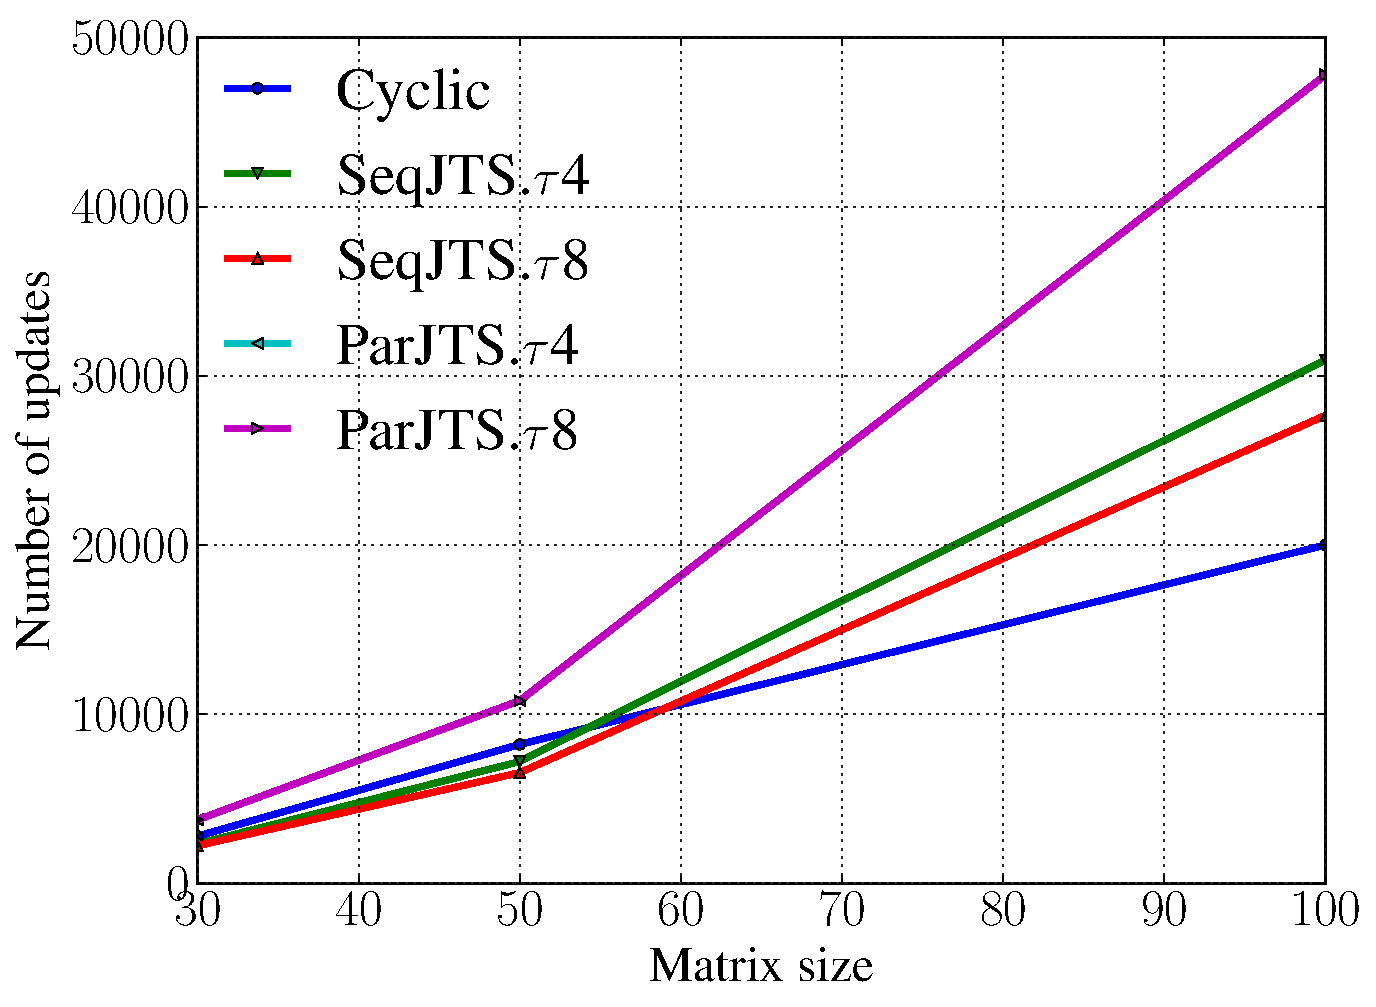
\includegraphics[width=0.48\textwidth]{updates}
 } \hfill
\subfloat[(b)][Time taken]{
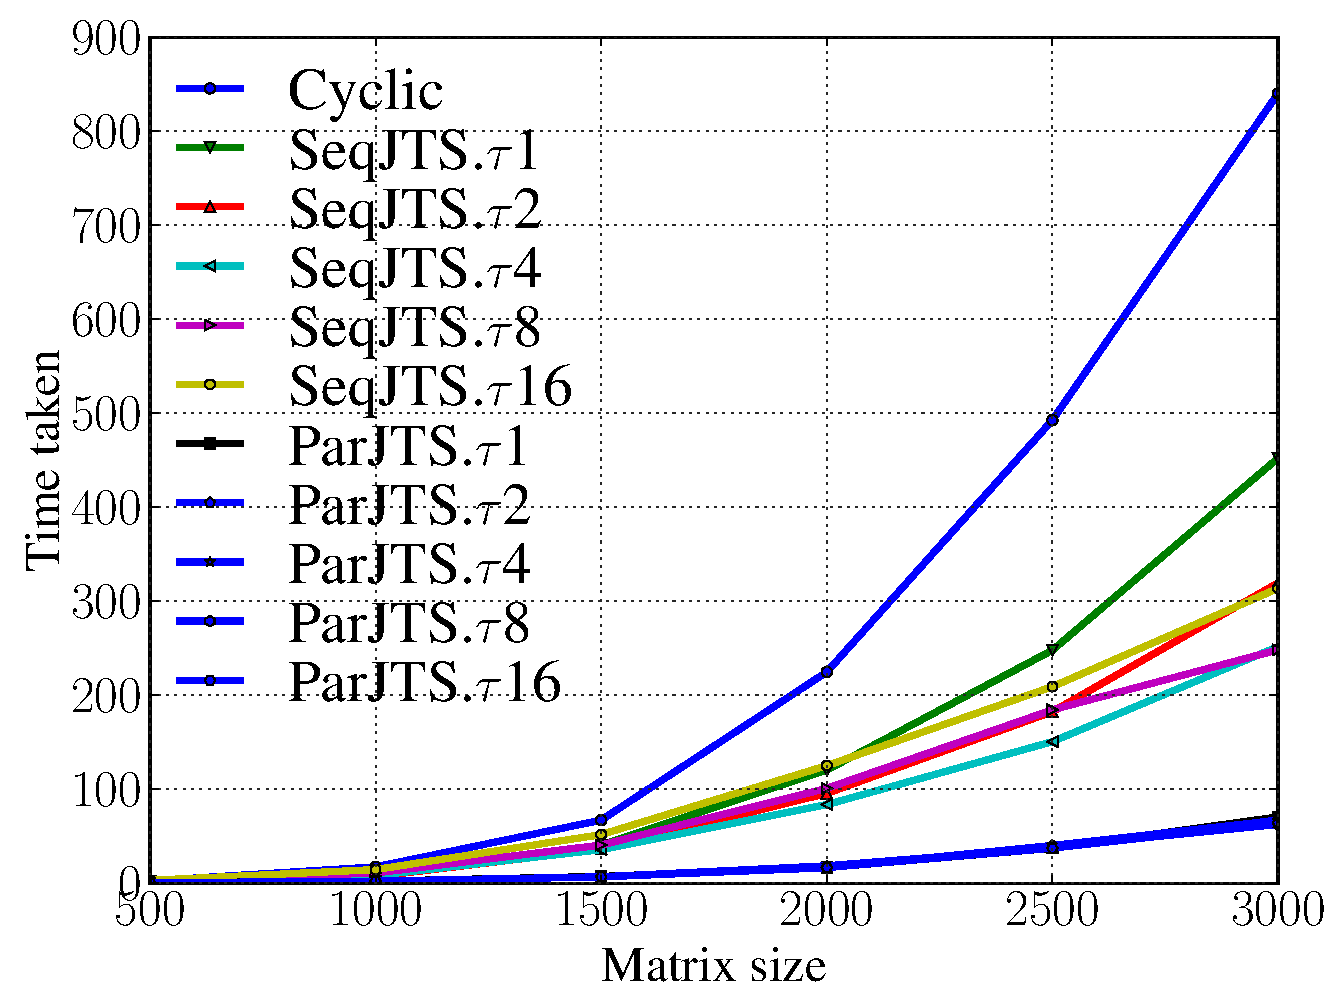
\includegraphics[width=0.48\textwidth]{timing}
 }
\caption{Performance of our parallel implementation}
\end{figure*}

\section{Implementation in Different Parallel Computing Models}
\label{sec:other}


\section{Conclusion}
\label{sec:conclude}

In this paper, we have proposed a novel algorithm (called
JRS Iteration Algorithm) for computing SVDs. This algorithm
enables us to perform all the rotations in a sweep independently
and in parallel without increasing the number of sweeps
significantly. Thus this algorithm can be implemented on a
variety of parallel models of computing to obtain optimal
speedups when the processor bound is O(n 2 ). This method
significantly decreases the number of sweeps over independent
Jacobi proposed in [11]. Therefore, our method can be used
in their stream algorithm to achieve a run time of O(nS). Our
algorithm can also be implemented on a CREW PRAM to have
a run time of O(S log 2 n). In this paper we have also provided
expressions for the relaxation parameter that will result in the
minimum number of sweeps.

%% use section* for acknowledgement
%\section*{Acknowledgment}
%
%
%The authors would like to thank...
%more thanks here
%
%\begin{table}[!t]
%% increase table row spacing, adjust to taste
%\renewcommand{\arraystretch}{1.3}
% if using array.sty, it might be a good idea to tweak the value of
% \extrarowheight as needed to properly center the text within the cells
%\caption{An Example of a Table}
%\label{table_example}
%\centering
%% Some packages, such as MDW tools, offer better commands for making tables
%% than the plain LaTeX2e tabular which is used here.
%\begin{tabular}{|c||c|}
%\hline
%One & Two\\
%\hline
%Three & Four\\
%\hline
%\end{tabular}
%\end{table}


% Note that IEEE does not put floats in the very first column - or typically
% anywhere on the first page for that matter. Also, in-text middle ("here")
% positioning is not used. Most IEEE journals/conferences use top floats
% exclusively. Note that, LaTeX2e, unlike IEEE journals/conferences, places
% footnotes above bottom floats. This can be corrected via the \fnbelowfloat
% command of the stfloats package.



% trigger a \newpage just before the given reference
% number - used to balance the columns on the last page
% adjust value as needed - may need to be readjusted if
% the document is modified later
%\IEEEtriggeratref{8}
% The "triggered" command can be changed if desired:
%\IEEEtriggercmd{\enlargethispage{-5in}}

% references section

\balance

% can use a bibliography generated by BibTeX as a .bbl file
% BibTeX documentation can be easily obtained at:
% http://www.ctan.org/tex-archive/biblio/bibtex/contrib/doc/
% The IEEEtran BibTeX style support page is at:
% http://www.michaelshell.org/tex/ieeetran/bibtex/
\bibliographystyle{IEEEtran}
% argument is your BibTeX string definitions and bibliography database(s)
\bibliography{IEEEabrv,jacobi}


% that's all folks
\end{document}


